\documentclass[tikz,convert={outfile=\jobname.svg}]{standalone}
%\usetikzlibrary{...}% tikz package already loaded by 'tikz' option
\usetikzlibrary{mindmap,trees}
\begin{document}
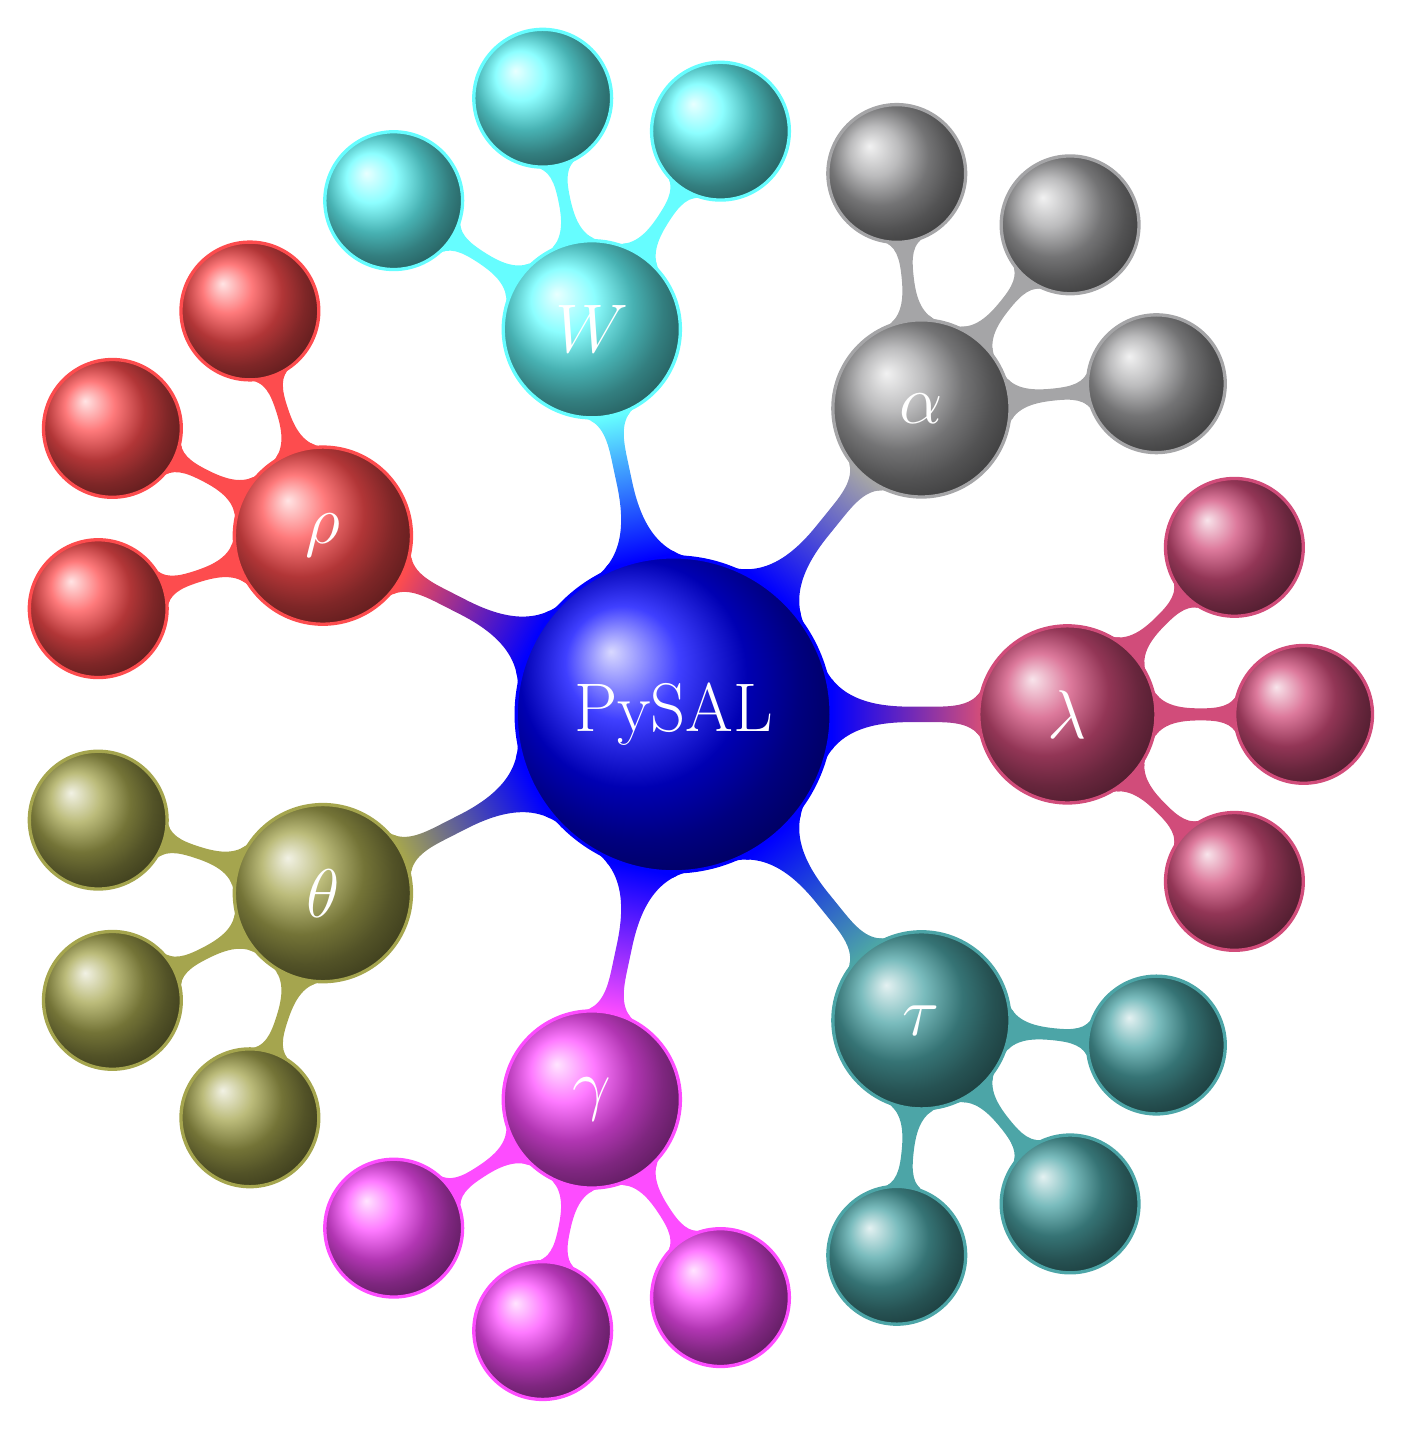
\begin{tikzpicture}[mindmap,
                    grow cyclic, 
                    every node/.style=concept, 
                    concept color=blue,
                    shading=ball,
                    text=white, 
                    level 1/.append style={level distance=5cm,
                                           sibling angle=51},
                    level 2/.append style={level distance=3cm,
                                           sibling angle=45},]
    \node[concept,ball color=blue]{\Huge{PySAL}}
	child [concept color=blue!1!olive!70]{ node [concept,ball color=blue!1!olive!70]{\Huge {$\theta$}}
		child [concept color=blue!1!olive!70]{ node [concept,ball color=blue!1!olive!70] { }}
		child [concept color=blue!1!olive!70]{ node [concept,ball color=blue!1!olive!70] { }}
		child [concept color=blue!1!olive!70]{ node [concept,ball color=blue!1!olive!70] { }}
	}
    	child [concept color=blue!1!magenta!70]{ node [concept,ball color=blue!1!magenta!70]{\Huge{$\gamma$}}
		child [concept color=blue!1!magenta!70]{ node [concept,ball color=blue!1!magenta!70] { }}
		child [concept color=blue!1!magenta!70]{ node [concept,ball color=blue!1!magenta!70] { }}
		child [concept color=blue!1!magenta!70]{ node [concept,ball color=blue!1!magenta!70] { }}
	}
	child [concept color=blue!1!teal!70]{ node [concept,ball color=blue!1!teal!70]{\Huge{$\tau$} }
		child [concept color=blue!1!teal!70]{ node [concept,ball color=blue!1!teal!70] { }}
		child [concept color=blue!1!teal!70]{ node [concept,ball color=blue!1!teal!70] { }}
		child [concept color=blue!1!teal!70]{ node [concept,ball color=blue!1!teal!70] { }}
	}
	child [concept color=blue!1!purple!70]{ node [concept,ball color=blue!1!purple!70]{\Huge{$\lambda$}}
		child [concept color=blue!1!purple!70]{ node [concept,ball color=blue!1!purple!70] { }}
		child [concept color=blue!1!purple!70]{ node [concept,ball color=blue!1!purple!70] { }}
		child [concept color=blue!1!purple!70]{ node [concept,ball color=blue!1!purple!70] { }}
	}
	child [concept color=blue!1!gray!70]{ node [concept,ball color=blue!1!gray!70]{\Huge{$\alpha$}}
		child [concept color=blue!1!gray!70]{ node [concept,ball color=blue!1!gray!70] { }}
		child [concept color=blue!1!gray!70]{ node [concept,ball color=blue!1!gray!70] { }}
		child [concept color=blue!1!gray!70]{ node [concept,ball color=blue!1!gray!70] { }}
	}
	child [concept color=blue!1!cyan!60]{ node [concept,ball color=blue!1!cyan!60]{\Huge{$W$}}
		child [concept color=blue!1!cyan!60]{ node [concept,ball color=blue!1!cyan!60] { }}
		child [concept color=blue!1!cyan!60]{ node [concept,ball color=blue!1!cyan!60] { }}
		child [concept color=blue!1!cyan!60]{ node [concept,ball color=blue!1!cyan!60] { }}
	}
	child [concept color=blue!1!red!70]{ node [concept,ball color=blue!1!red!70]{\Huge{$\rho$} }
		child [concept color=blue!1!red!70]{ node [concept,ball color=blue!1!red!70] { }}
		child [concept color=blue!1!red!70]{ node [concept,ball color=blue!1!red!70] { }}
		child [concept color=blue!1!red!70]{ node [concept,ball color=blue!1!red!70] { }}
	}
    	;
\end{tikzpicture}
\end{document}